\section{Principles for building a modern and flexible data architecture for official statistics}
\label{sec:principles}

With the emergence of big data sources and new methodologies offering significant promise to improve the production process of official statistics, statisticians trained in data science techniques are eager to innovate. However, their ability to do so is limited by several challenges. Central among these challenges is the need for greater autonomy — be it in scaling resources to match statistical workloads, deploying proofs of concept with agility and in a collaborative manner, etc. Against this background, our aim was to design a data science platform that not only manages big data efficiently but also empowers statisticians by enhancing their autonomy. To achieve this, we delved into the evolving data ecosystem in order to identify significant trends with the potential to overcome the aforementioned limitations\footnote{As a preamble to this review, we should note that, although we did our best to ground our insights in the academic literature, a lot of it stems from informal knowledge  gathered through diligent and ongoing technology watch. In the rapidly evolving data ecosystem, traditional research papers are increasingly giving way to blog posts as the primary references for cutting-edge developments. This shift is largely due to the swift pace at which big data technologies and methodologies are advancing, making the lengthy publication process of formal research often not the preferred way of disseminating timely insights and innovations.}. Our findings indicate that leveraging cloud-native technologies, particularly containers and object storage, is key to building infrastructures capable of handling large and varied datasets in a flexible, cost-effective manner. Furthermore, these technologies significantly enhance autonomy, facilitating innovation and promoting reproducibility in the production of official statistics.

\subsection{Limitations of traditional big data architectures}

Over the last decade, the landscape of big data has dramatically transformed. Following the publication of Google's seminal papers that introduced the MapReduce paradigm \cite{ghemawat2003google, dean2008mapreduce}, Hadoop-based systems rapidly became the reference architecture of the big data ecosystem, celebrated for their capability to manage extensive datasets through the use of distributed computing. The inception of Hadoop marked a revolutionary step, enabling organizations to process and analyze data at an unprecedented scale. Basically, Hadoop provided companies with all-rounded capabilities for big data analytics: tools for ingestion, data storage (HDFS), and computing capacities (Spark, among others) \cite{dhyani2014big}, thus explaining its rapid adoption across industries.

In the late 2010's, Hadoop-based architectures have experienced a clear decline in popularity. In traditional Hadoop environments, storage and compute were co-localized by design: if the source file is distributed across multiple servers (horizontal scaling), each section of the source file is directly processed on the machine hosting that section, so as to avoid network transitions between servers. In this paradigm, scaling the architecture often meant a linear increase in both compute and storage, regardless of the actual demand. In a recent article provocatively titled "Big Data is Dead"\footnote{\url{https://motherduck.com/blog/big-data-is-dead/}}, Jordan Tigani, one of the founding engineers behind Google BigQuery, explains why this model doesn't fit the reality of most data-centric organizations anymore. First, because "in practice data sizes increase much faster than compute sizes". While the amount of data generated and thus needing to be stored may grow linearly over time, it is generally the case that we only need to query the most recent portions of it, or only some columns and/or groups of rows. Besides, Tigani points out that "the big data frontier keeps receding": advancements in server computing capabilities and declining hardware costs mean that the number of workloads that don't fit on a single machine — a simple yet effective definition of big data — has been continually decreasing. As a result, by properly separating storage and compute functions, even substantial data processing jobs may end up using "far less compute than anticipated [...] and might not even need to use distributed processing at all".

These insights strongly align with our own observations at Insee in recent years. As a use case of using big data infrastructures to improve statistical processes, an Insee team set up a Hadoop cluster as an alternative architecture to the one already in use to process sales receipt data in the context of computing the consumer price index. An acceleration of data processing operations by up to a factor of 10 was achieved, for operations that previously took several hours to perform \cite{leclair2019utiliser}. Despite this increase in performance, this type of architectures were not reused later for several reasons. Mainly, the architecture proved to be expensive and complex to maintain, necessitating specialized technical expertise rarely found within NSOs \cite{vale2015international}. But interestingly, subsequent projects involving large datasets didn't suffer much from this change, as their needs were actually very much in line with Tigani's observations. The bottleneck for these projects was generally on the side of computational needs rather than storage capacity. Furthermore, although these projects could still involve substantial data volumes, we observed that effective processing could be achieved using conventional software tools (R, Python) on single-node systems by leveraging recent important innovations from the data ecosystem. First, by using efficient formats to store the data such as Apache Parquet \cite{parquet2013}, which properties — columnar storage \cite{abadi2013design} (see figure\ref{fig:columnar-storage}), optimisation for the "write once, read many" (WORM) paradigm, ability to partition data, etc. — make it particularly suited to analytical tasks such as those generally performed in official statistics \cite{abdelaziz2023optimizing}. Second, by performing computations using optimised in-memory computation frameworks such as Apache Arrow \cite{arrow2016} or DuckDB \cite{raasveldt2019duckdb}. Also based on columnar representation — thus working in synergy with Parquet files — both of these frameworks greatly improve data queries performance through the use of "lazy evaluation": instead of doing lots of separate operations (e.g. selecting columns and/or filtering rows, then computing new columns, then performing agregations, etc.), they process them all at once in a more optimised way. As a result, computations are limited to the data effectively needed by the queries, enabling much larger-than-memory data processing on usual single-node machines.

\begin{figure}[htbp]
    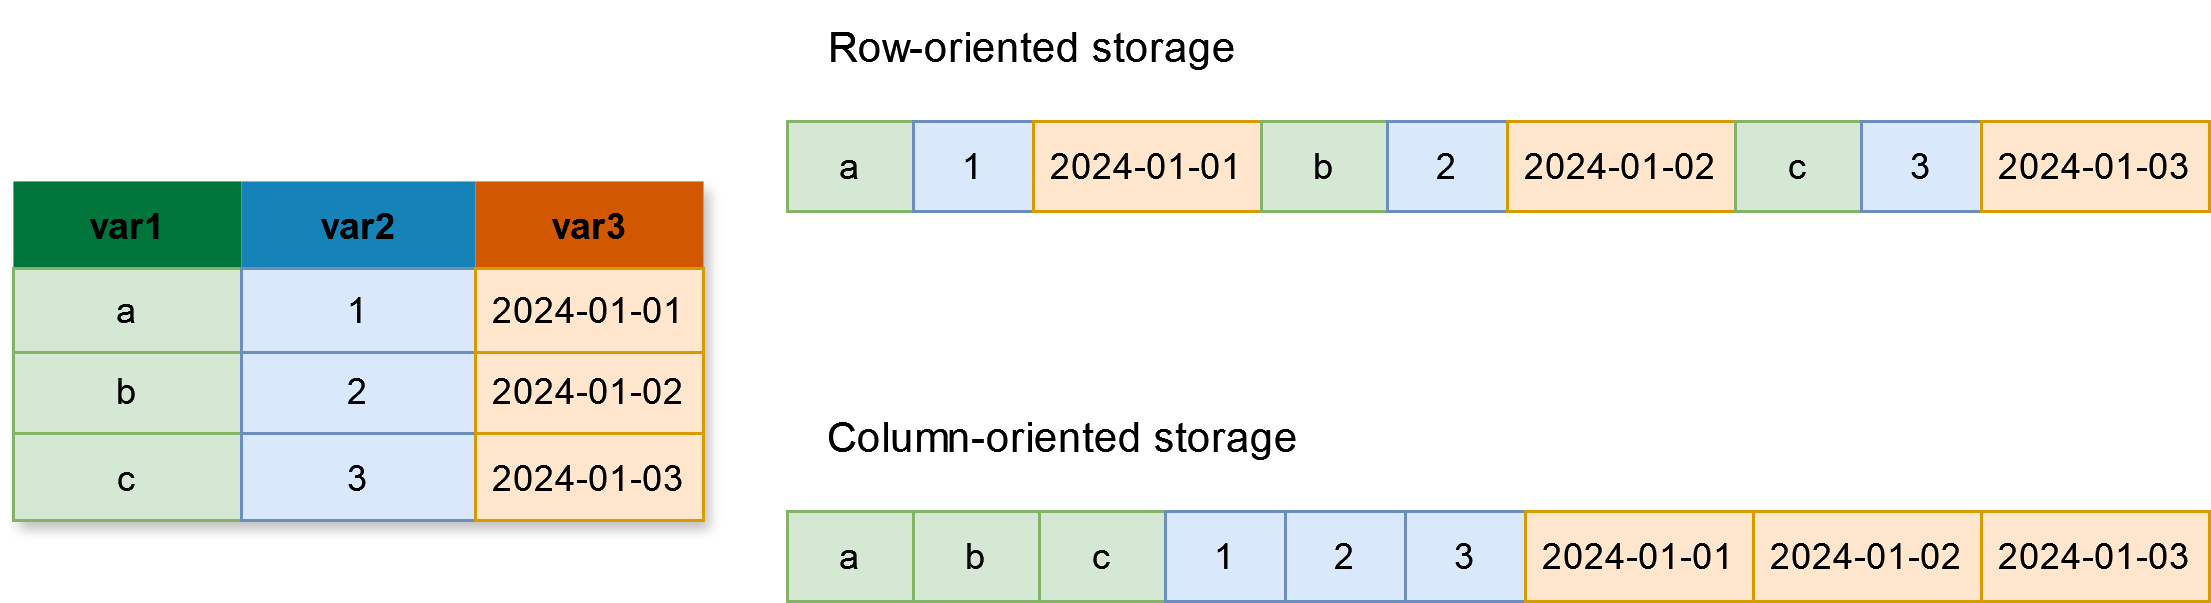
\includegraphics[width=\linewidth]{sections/img/columnar-storage.png}
    \caption{Row-oriented and column-oriented representation of a same dataset.}
    \label{fig:columnar-storage}
    \medskip
    {\footnotesize Note: Many statistical operations are analytical (OLAP) in nature: they involve selecting specific columns, computing new variables, performing group-based aggregations, etc. Row-oriented storage is not well-suited to analytical operations as it requires the full dataset to be read in memory to query it. Conversely, column-based storage allows only relevant data columns to be queried, significantly reducing read and processing times for analytical workloads. In practice, popular columnar formats such as Parquet use a hybrid-representation: they are primarily column-oriented but also implement clever row-based grouping to optimize filtering queries.}
\end{figure}

\subsection{Embracing cloud-native technologies}

In light of this evolution of the big data ecosystem, there has been a notable shift in recent years within the industry towards more flexible and loosely coupled architectures. The advent of cloud technologies has been instrumental in facilitating this shift. Unlike the era where Hadoop was prominent, network latency has become much less of a concern, making the traditional model of on-premise and co-located storage and compute solutions less relevant. In terms of the nature of the data that need to be processed, we are observing an evolution that some have described as moving "from big data to flexible data": modern data infrastructures are required not only to process large volumes but also to be adaptable in multiple dimensions: accommodating various data structures (ranging from structured, tabular formats to unstructured formats like text and images), ensuring data portability across multi-cloud and hybrid cloud environments, and supporting a diverse range of computational workloads (from parallel computations to deep learning models necessitating GPUs, as well as the deployment and management of applications) \cite{li2020big}. In recent years, two technologies have emerged in the data ecosystem as foundational technologies for achieving such flexibility in cloud-based environments: containerization and object storage. 

In a cloud environment, the computer of the user becomes a simple access point to perform computations on a central infrastructure. This enables both ubiquitous access to and scalability of the services, as it is easier to scale a central infrastructure — usually horizontally, i.e. by adding more servers. However, such centralized infrastructures have two well-identified limitations that need to be dealt with: the competition between users in access to physical resources and the need to properly isolate deployed applications. The choice of containerization is fundamental as it tackles these two issues \cite{bentaleb2022containerization}. By creating “bubbles” specific to each service, containers guarantee application isolation while remaining lightweight, as they share the support operating system with the host machine (see. graph\ref{fig:containers}). In order to manage multiple containerized applications in a systematic way, containerized infrastructures generally rely on an orchestrator software — the most prominent one being Kubernetes, an open-source project initially developed by Google to manage its numerous containerized workloads in production \cite{vano2023cloud}. Orchestrators automate the process of deploying, scaling, and managing containerized applications, coordinating their execution across various servers. Interestingly, this property makes it possible to handle very large volumes of data in a distributed way: containers break down big data processing operations into a multitude of small tasks, organized by the orchestrator. This minimizes the required resources while providing more flexibility than hadoop-based architectures \cite{zhang2018comparative}.

\begin{figure}[htbp]
    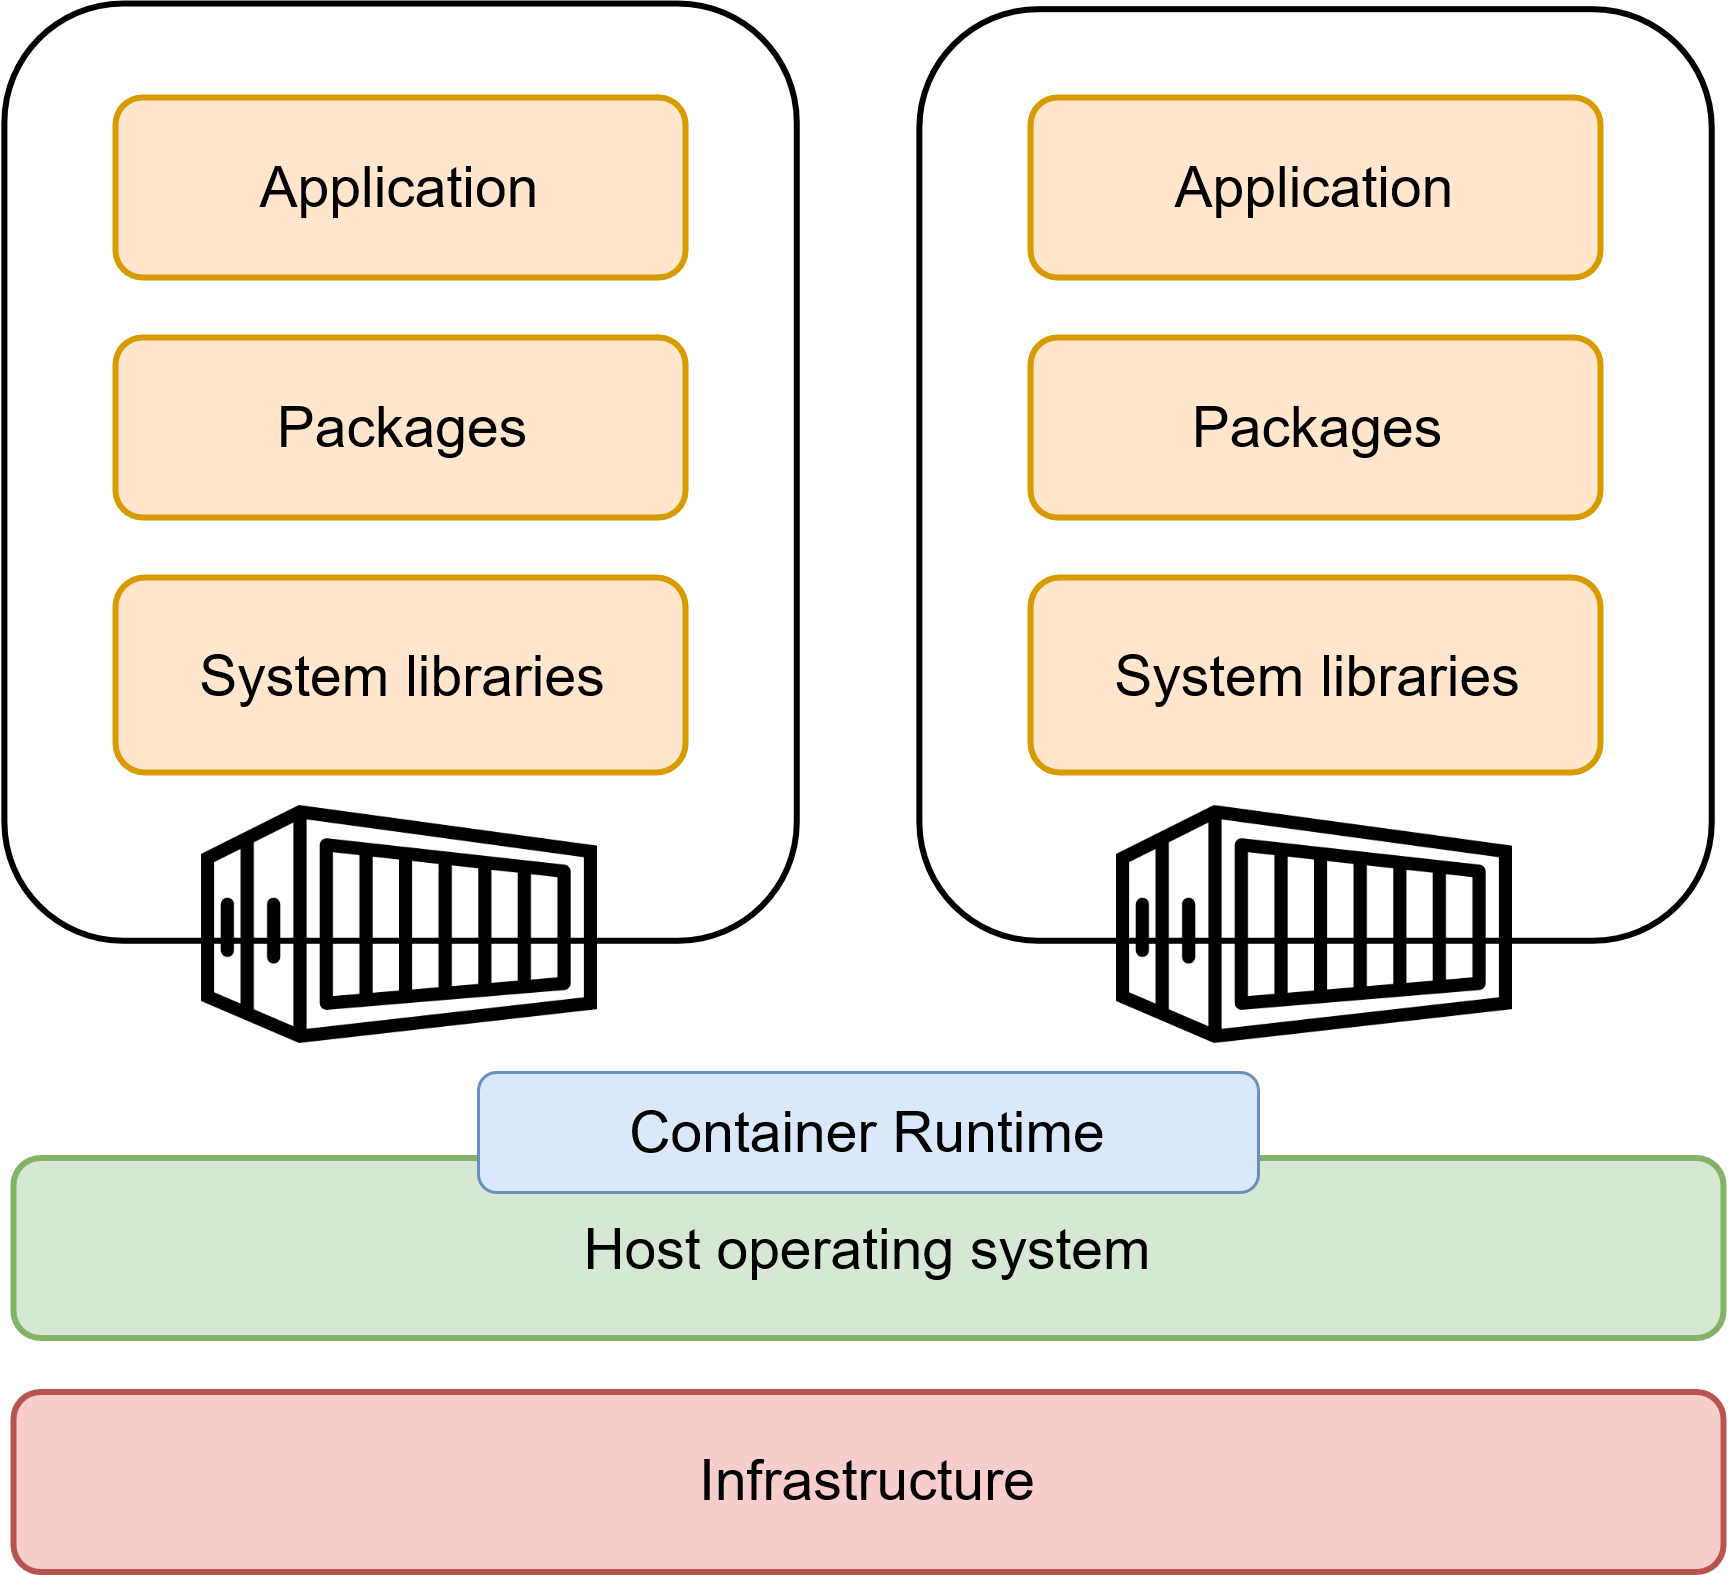
\includegraphics[width=\linewidth]{sections/img/containers.png}
    \caption{Architecture of a containerized environment.}
    \label{fig:containers}
    \medskip
    {\footnotesize Note: A container is a logical grouping of resources that makes it possible to encapsulate an application (e.g. Python code), the packages used (e.g. Pandas, NumPy) and system libraries (the Python interpreter, other OS-dependent libraries, etc.), in a single package. Containerized applications are isolated from one another through virtualization, which makes it possible to attribute specific physical resources to each application while guaranteeing complete independence between them. But contrary to virtual machines which also virtualize the operating system (OS), containers rely on a lightweight form of virtualization: the container shares the OS of the host infrastructure through the container runtime (e.g. Docker). As a result, containers are much more portable and can be readily deployed and redistributed.}
\end{figure}

The other fundamental choice in a data architecture is the nature of data storage. In the cloud ecosystem, so-called "object storage" has become the de-facto reference \cite{samundiswary2017object} \footnote{Mainly because of Amazon's "S3" (Simple Storage Service) implementation.}. In this paradigm, files are stored as "objects" consisting of data, an identifier and metadata. This type of storage is optimized for scalability, as objects are not limited in size and the underlying technology enables cost-effective storage of (potentially very) large files. It is also instrumental in building a decoupled infrastructure such as discussed before: the data repositories — referred to as "buckets" — are directly searchable using standard HTTP requests through a standardized REST API. In a world where network latency is not the main bottleneck anymore, this means that storage and compute don't have to be on the same machines or even in the same location, and can thus scale independently according to specific organization demands. Finally, object storage is a natural complement to architectures based on containerized environments for which it provides a persistence layer — containers being stateless by design — and easy connectivity without compromising security, or even with strengthened security compared with a traditional storage system \cite{mesnier2003object}.

\subsection{Leveraging cloud technologies to increase autonomy and foster reproducibility}

Understanding how the technological choices described in the technical discussion above are relevant in the context of official statistics require an in-depth review of statisticians’ professional practices in their use of computing environments. At the end of the 2000s, with micro-computing at its peak, many of the technical resources used by statisticians at Insee were local: the code and processing software were located on individual computers, while data was accessed through a file-sharing system. Because of the the limited scalability of personal computers, this setup greatly limited the ability of statisticians to experiment with big data sources or computationally intensive statistical methods, and involved security risks because of the widespread data dissemination within the organization. In order to overcome these limitations, a transition was made towards centralised IT infrastructures, concentrating all — and thus overall much more — resources on central servers. Such infrastructures, made available to statisticians through a shared, virtual desktop environment for ease of use, remains the dominant method for conducting statistical computations at Insee at the time of writing this lines.

Through our observations and discussions with fellow statisticians, it became evident that although the current IT infrastructure adequately supported the core activities of statistical production, it noticeably restricted statisticians' capacity to experiment freely and innovate. The primary bottleneck in this organization is the dependency of statistical projects on centralized IT decision-making, such as the allocation of computing resources, access to shared data storage, the use of pre-configured programming languages and packaging environments, etc. Besides, such dependencies often lead to a well-known phenomenon within the software development community that lies at the heart of the DevOps approach, where the priorities of developers — iterate rapidly to improve functionality in a continuous manner — often clash with IT's focus on security and process stability. On the contrary, it is our understanding that modern data science practices reflect an increased involvement of statisticians in the IT development and orchestration of their data processing operations, beyond merely the design or validation phases. New data science infrastructures must take this expanded role of their users into account, giving them more autonomy than conventional infrastructures.

Cloud technologies stand out as a powerful solution to grant statisticians this much-needed autonomy in their daily work, enabling a culture of innovation. Through object storage, users gain control over the storage layer, allowing them to experiment with diverse datasets without being constrained by the limited storage spaces typically allocated by IT departments. Containerization empowers users to customize their working environments to their specific needs — be it programming languages, system libraries, or package versions — while also providing the flexibility to scale their applications according to the required computing power and storage capacities. By design, containers also foster the development of portable applications, which enables smoother transitions between environments (development, qualification, production), ensuring that applications can be moved seamlessly without the hurdles of environmental inconsistencies. Finally, with orchestration tools like Kubernetes, statisticians can more readily deploy applications and APIs and automatize the whole building process, sidestepping complexities associated with inconsistent or complex deployment environments. This capability aligns with the DevOps approach, enabling quicker iteration and building minimal prototypes as proofs of concept (POCs) rather than building the optimal (but time-consuming) solution for a pre-defined objective \cite{leite2019survey}.

% TODO: figure diagram object storage + compute -> reproductible outputs

Besides scalability and autonomy, these architectural choices also foster reproducibility of statistical computations. The concept of reproducibility — namely the ability to reproduce the result of an experiment by applying the same methodology to the same data — is a fundamental criterion of scientific validity \cite{mcnutt2014reproducibility}. It is also highly relevant in official statistics, as it serves as a foundation for transparency, which in turn is crucial for building and maintaining the public's trust. Fostering reproductibility in statistical production involves devising processing solutions that can produce reproducible statistics on the one hand, and that can be shared with peers on the other hand \cite{ntts2019reproducibility}. Traditional IT infrastructures — either a personal computer or a shared infrastructure with remote desktop access — fall short in this regard, as building a project or just computing a statistical indicator there generally involves a series of manual steps (installing system libraries, the programming language binary, projects packages, dealing with potentially conflicting versions, etc.) that can not be fully reproduced across projects. In comparison, containers are reproducible by design, as their build process involves defining precisely all the needed resources as a set of processing operations in a standardized manner, from the "bare machine" to the running application \cite{moreau2023containers}. Furthermore, these reproducible environments can be easily shared to peers as they can be readily published on open registries (for example, a container registry such as DockerHub) along to the source code of the application (for example, on a public software forge like GitHub or GitLab). This approach significantly enhances the reusability of code projects, fostering a community-driven model of development and innovation.
